\chapter{Página de Internet}\label{chap:webpage}

	Como se comentó en el capítulo de introducción una gran ventaja del lenguaje java es su capacidad para crear páginas de internet. En el presente trabajo se creó una página de internet cuyo objetivo es exponer las funciones principales de la librería materia.

	La página se encuentra en la dirección web: \url{chimicae-materia.rhcloud.com}, se recomienda utilizar un navegador moderno como google chrome.

	El presente capítulo trata sobre como utilizar la página para:

	\begin{itemize}
		\item{Crear}
			\begin{itemize}
				\item{Substancias} Sección \ref{sec:webSubstanceCreator}
				\item{Mezclas} Sección \ref{sec:webMixtureCreator}
			\end{itemize}
		\item{Gráficas}
			\begin{itemize}
				\item \nameref{subsec:pvt}
				\item \nameref{subsec:zpt}
				\item \nameref{subsec:fpt}
				\item \nameref{subsec:tep}
				\item \nameref{subsec:tsp}
				\item \nameref{subsec:tgp}
				\item \nameref{subsec:tpv}
			\end{itemize}
		\item{Estimación de parámetros}
			\begin{itemize}
				\item Expresión de $\alpha$
				\item Regla de Mezclado
			\end{itemize}
	\end{itemize}

\section{Selección de compuestos puros}\label{sec:webCompounds}

	La página de internet dispone de la base de datos ChemSep v6.96 derechos de autor  Harry Kooijman y Ross Taylor (2013) bajo la licencia `Artistic License': \url{ http://www.perlfoundation.org/artistic_license_2_0}.

	Primero se debe cargar los compuestos puros, en la sección `Creación' -> `Compuesto Puro', en el recuadro de texto se debe escribir el nombre del compuesto puro deseado en inglés y dar click en el boton buscar. Si la página encuentra coincidencia en los nombre mostrará una lista debajo del recuadro con los compuestos encontrados.

	Para agregar el compuesto basta con dar click en el boton `Agregar' .En la tabla que se muestra a la derecha de la página se muestran los compuestos agregados. Ver la figura \ref{fig:pureCompounds}.

	\begin{figure}
		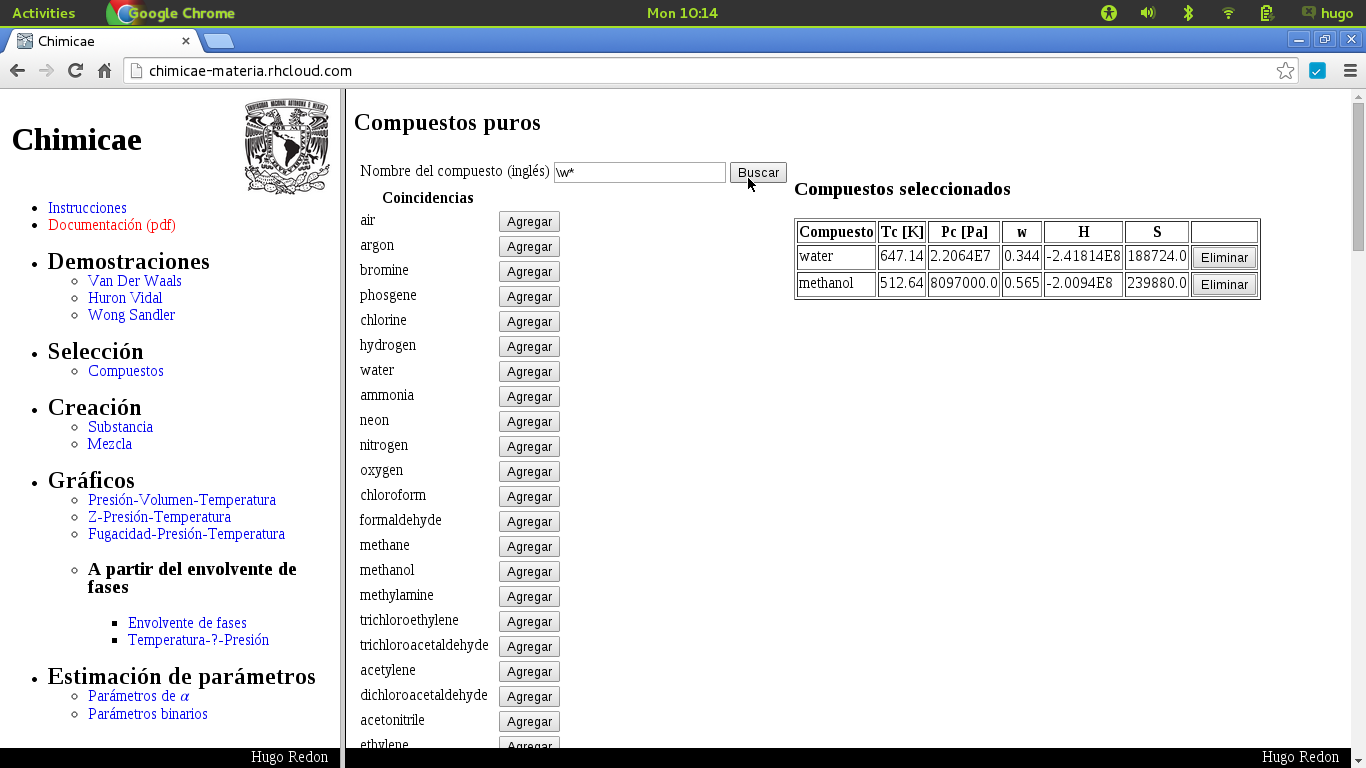
\includegraphics[scale=0.3]{pureCompounds.png}
		\caption{Formulario para seleccionar y cargar compuestos puros en la página de internet}
		\label{fig:pureCompounds}
	\end{figure}

\section{Creación de substancias}\label{sec:webSubstanceCreator}
	
	En la sección `Creación' -> `Substancia' se permite crear materia de un solo compuesto, para después utilizarse en las secciones de graficación y estimación de parámetros de la expresión de $\alpha$.

	Esta sección permite elegir la ecuación cúbica, la expresión de $\alpha$,el compuesto y la fase homogéna con la cual se creará la substancia. Al final de la sección el botón `Aceptar' creará la Substancia y mostrará el resultado de la creación.

	La figura \ref{fig:substanceCreator} muestra la interfaz de usuario para la creación de substancias. La figura \ref{fig:substanceProperties} muestra las propiedades de la substancia creada.

	\begin{figure}
		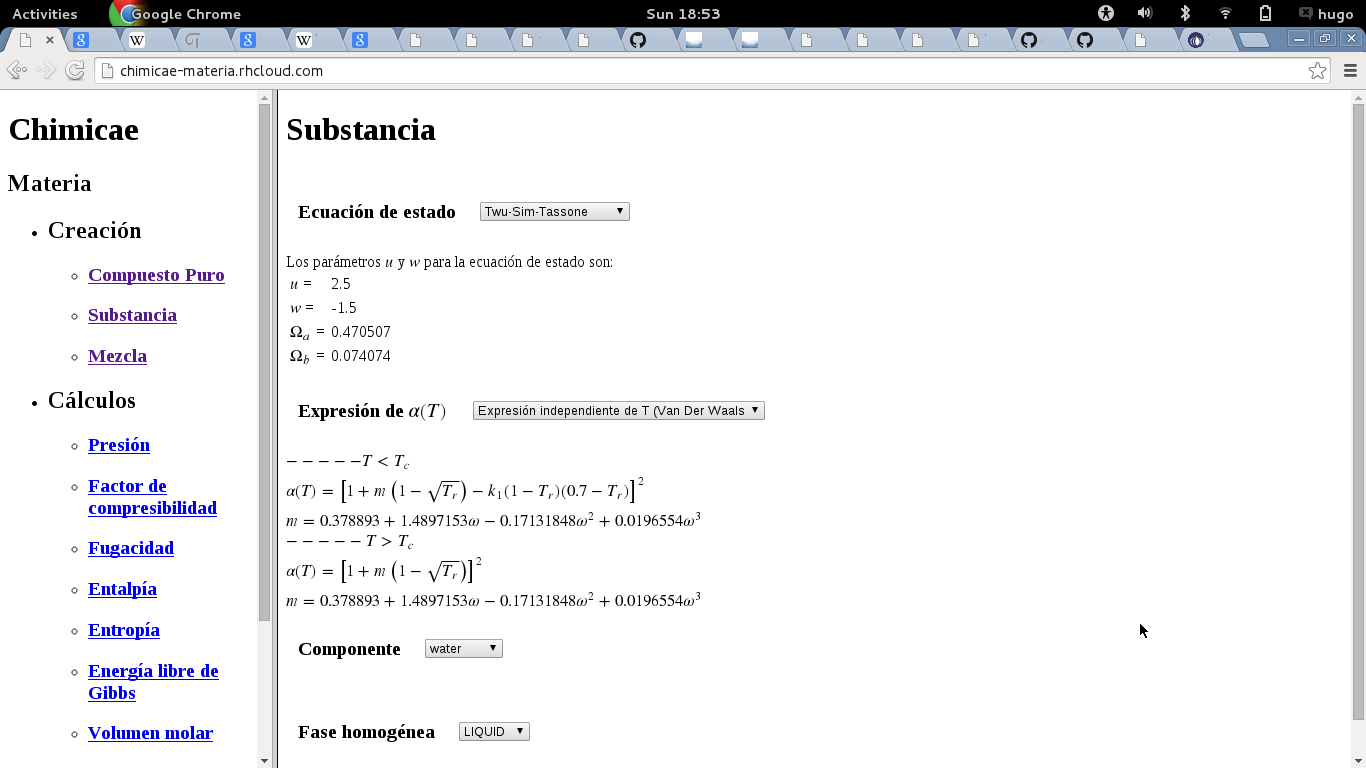
\includegraphics[scale=0.3]{substanceCreator.png}
		\caption{Formulario para crear substancias en la página de internet}
		\label{fig:substanceCreator}
	\end{figure}

	\begin{figure}
		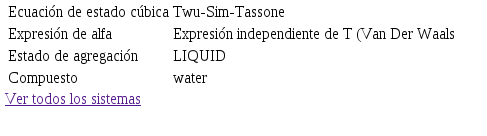
\includegraphics[scale=0.3]{substanceProperties.png}
		\caption{Página que muestra las propiedades de la substancia recien creada}
		\label{fig:substanceProperties}
	\end{figure}

\section{Creación de Mezclas}\label{sec:webMixtureCreator}

	En la sección `Creación' -> `Mezcla' que permite crear materia con multiples compuestos puros, solo aquellas mezclas que contengan dos compuestos estarán disponibles en la sección \nameref{sec:webBinaryOptim}.

	El formulario permite elegir la ecuación cúbica, la fase ,la regla de mezclado, elegir cada compuesto y definir su expresión de $\alpha$ y su fración molar. Ver figura \ref{fig:webMixCreator}.

	\begin{figure}
		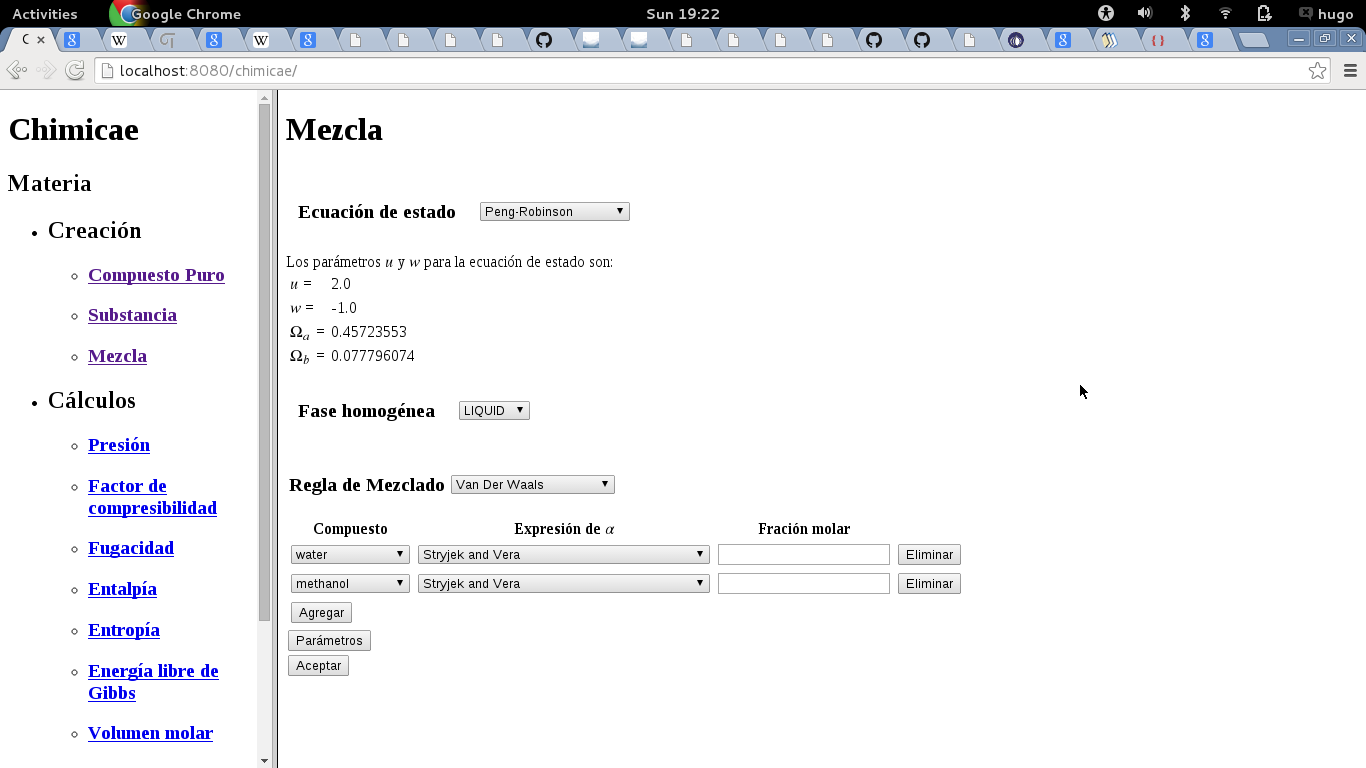
\includegraphics[scale=0.3]{mixtureCreator.png}
		\caption{Formulario para la creación de mezclas}
		\label{fig:webMixCreator}
	\end{figure}

	El botón con la etiqueta `Parámetros' permite definir los parámetros binarios para la regla de mezclado seleccionada. Finalmente el botón `Aceptar' construye la mezcla y la pone a disposición para las siguientes secciones.

\section{Gráficos}

	En la sección `Gráficos' de la página de internet estan disponibles las substancias y mezclas creadas anteriormente, basta con selecciónar y dar click en el botón para ver la gráfica.

	En algunas gráficas se muestran los resultados de la fase líquida y vapor sin importar que fase se le haya dado al sistema en el momento de su creación.

	\subsection{Presión-Volumen-Temperatura}\label{subsec:pvt}
		\begin{figure}[!h]
			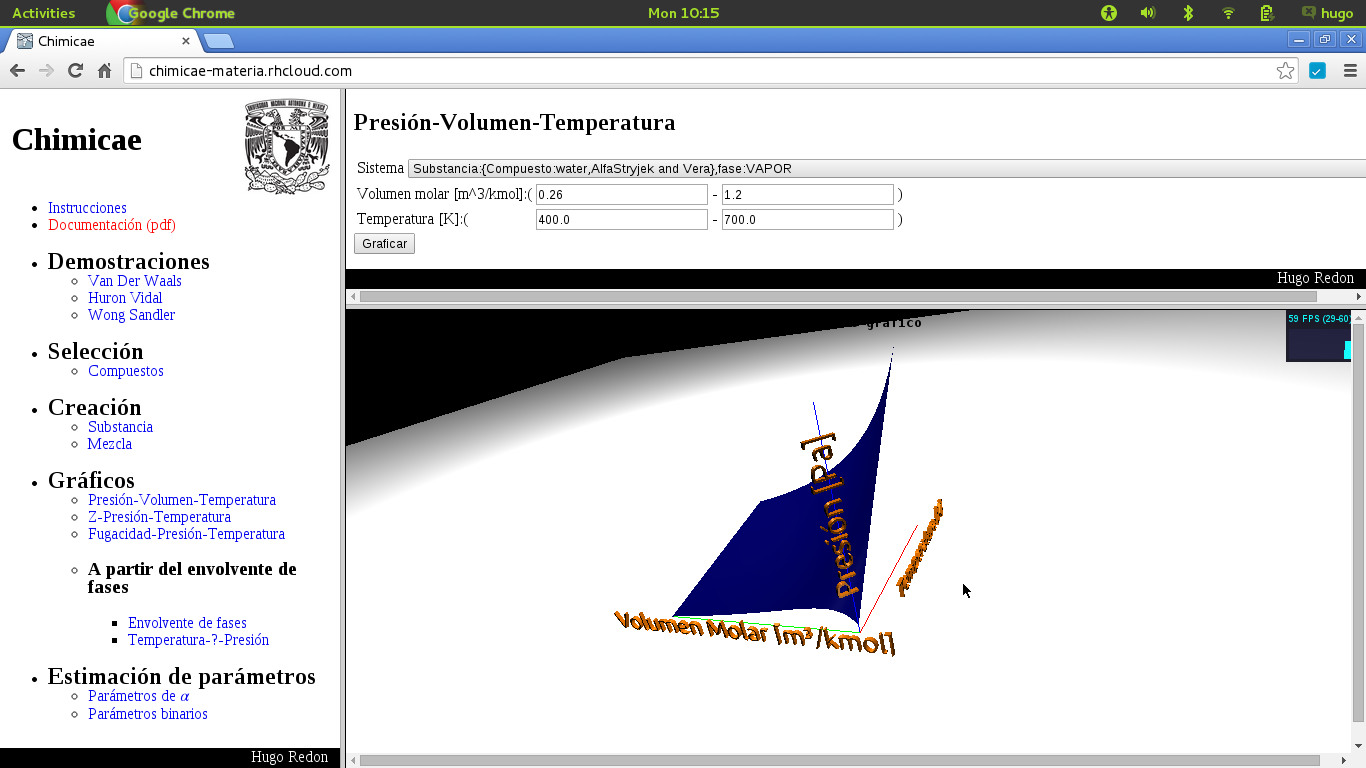
\includegraphics[scale=0.3]{waterPressurePlot.png}
		\end{figure}
	\subsection{Z-Presión-Temperatura}\label{subsec:zpt}
		\begin{figure}[!h]
			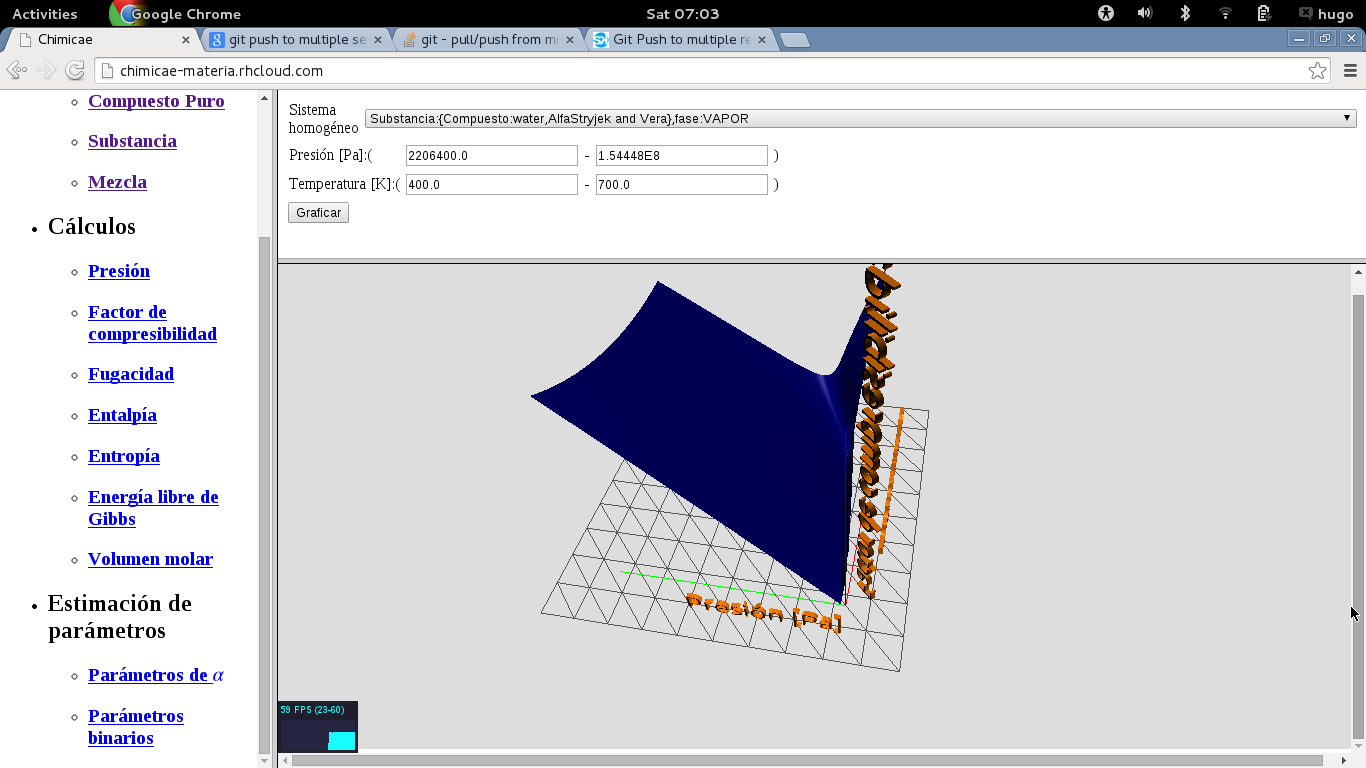
\includegraphics[scale=0.3]{waterZPlot.png}
		\end{figure}
	\subsection{Fugacidad-Presión-Temperatura}\label{subsec:fpt}
		\begin{figure}[!h]
			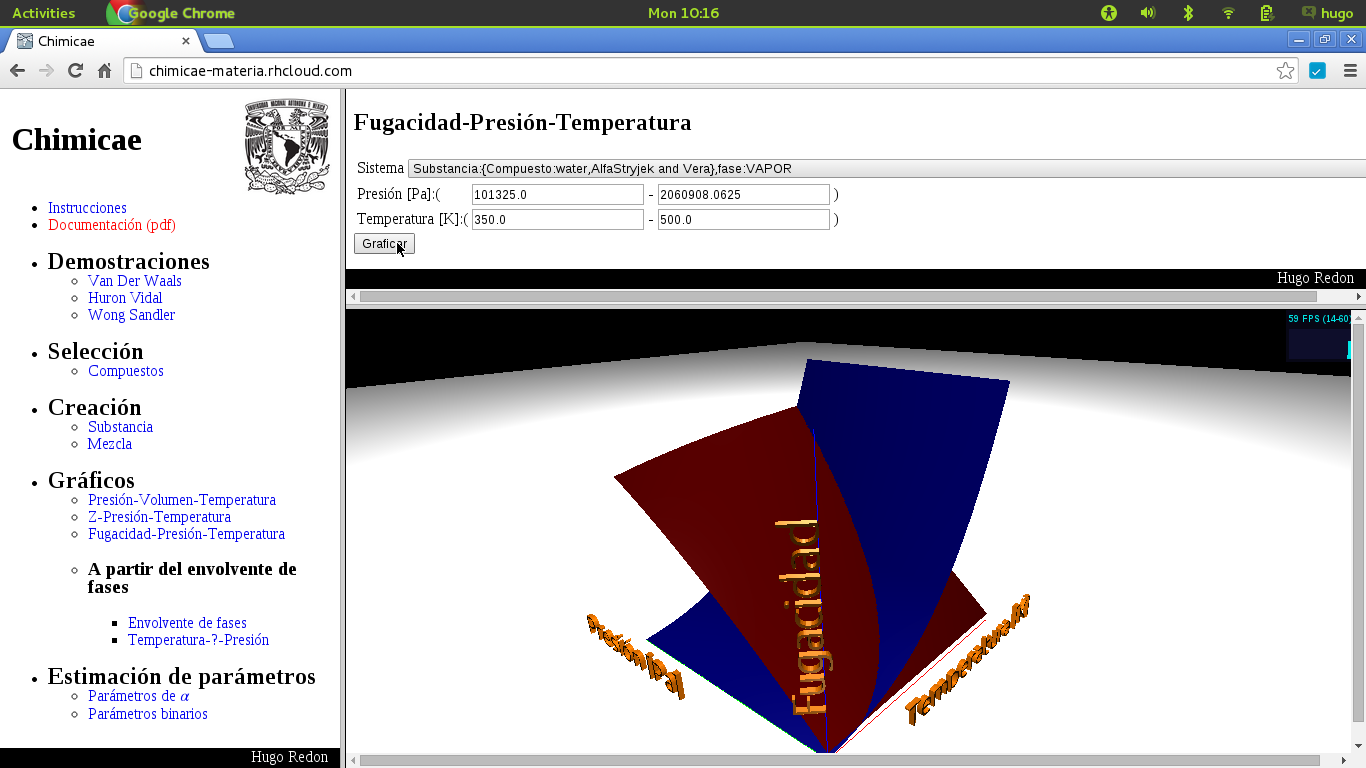
\includegraphics[scale=0.3]{waterFugacityPlot.png}
		\end{figure}
	\subsection{Temperatura-Entalpía-Presión}\label{subsec:tep}
		\begin{figure}[!h]
			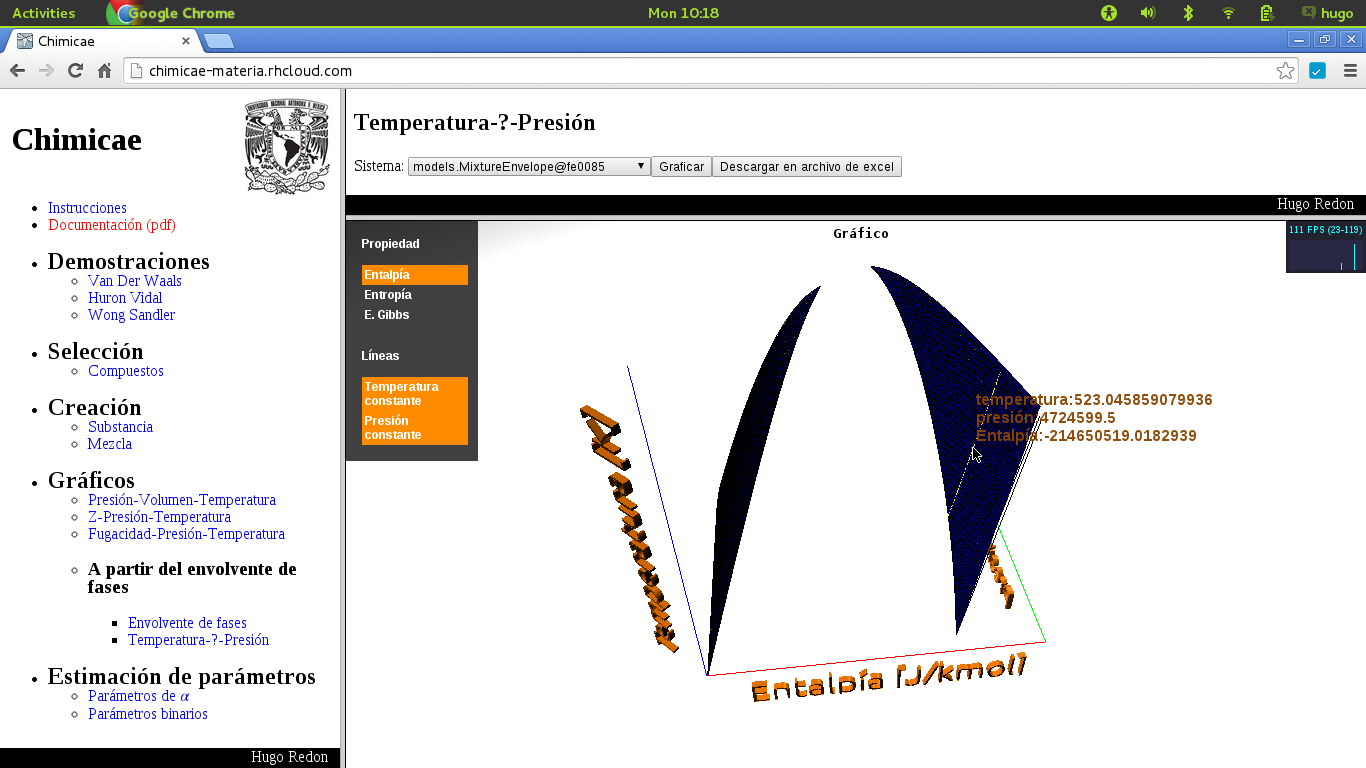
\includegraphics[scale=0.3]{waterEnthalpyPlot.png}
		\end{figure}
	\subsection{Temperatura-Entropía-Presión}\label{subsec:tsp}
		\begin{figure}[!h]
			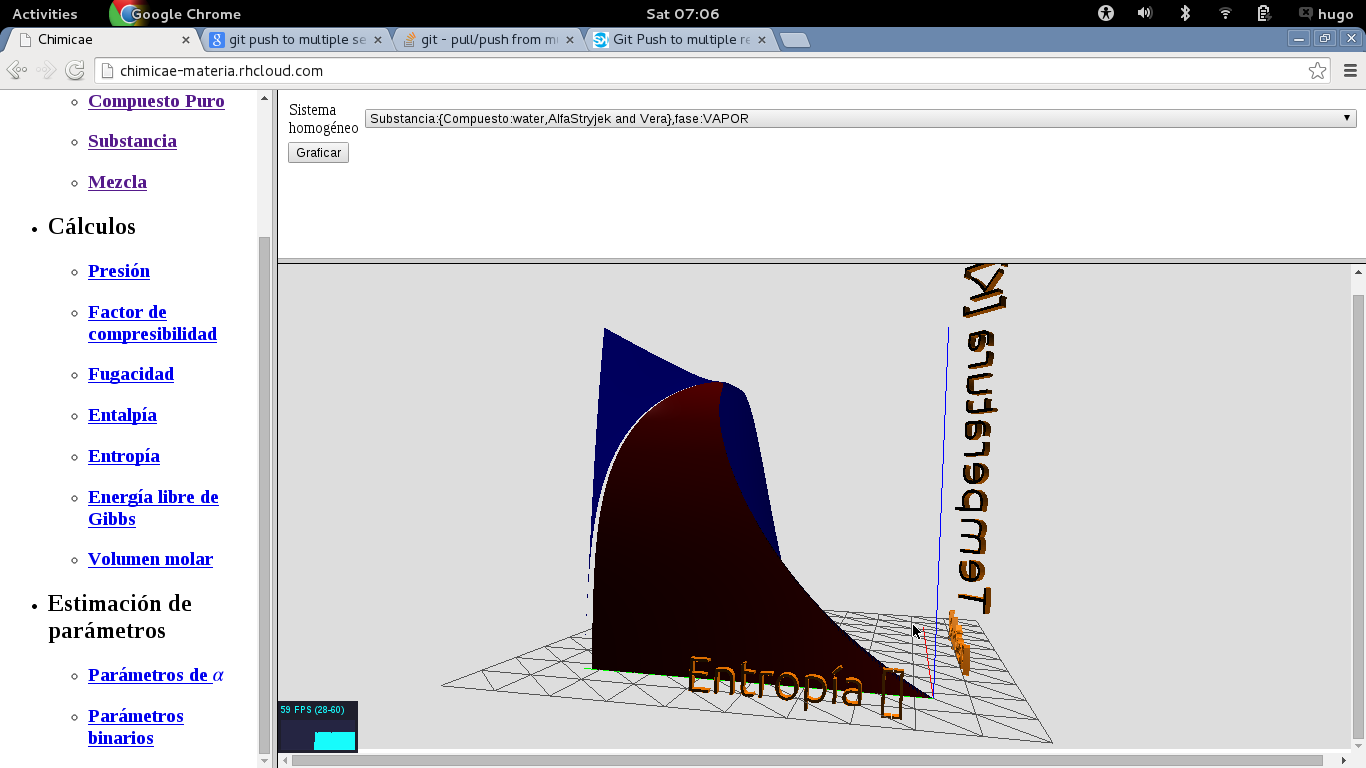
\includegraphics[scale=0.3]{waterEntropyPlot.png}
		\end{figure}
	\subsection{Temperatura-Gibbs-Presión}\label{subsec:tgp}
		\begin{figure}[!h]
			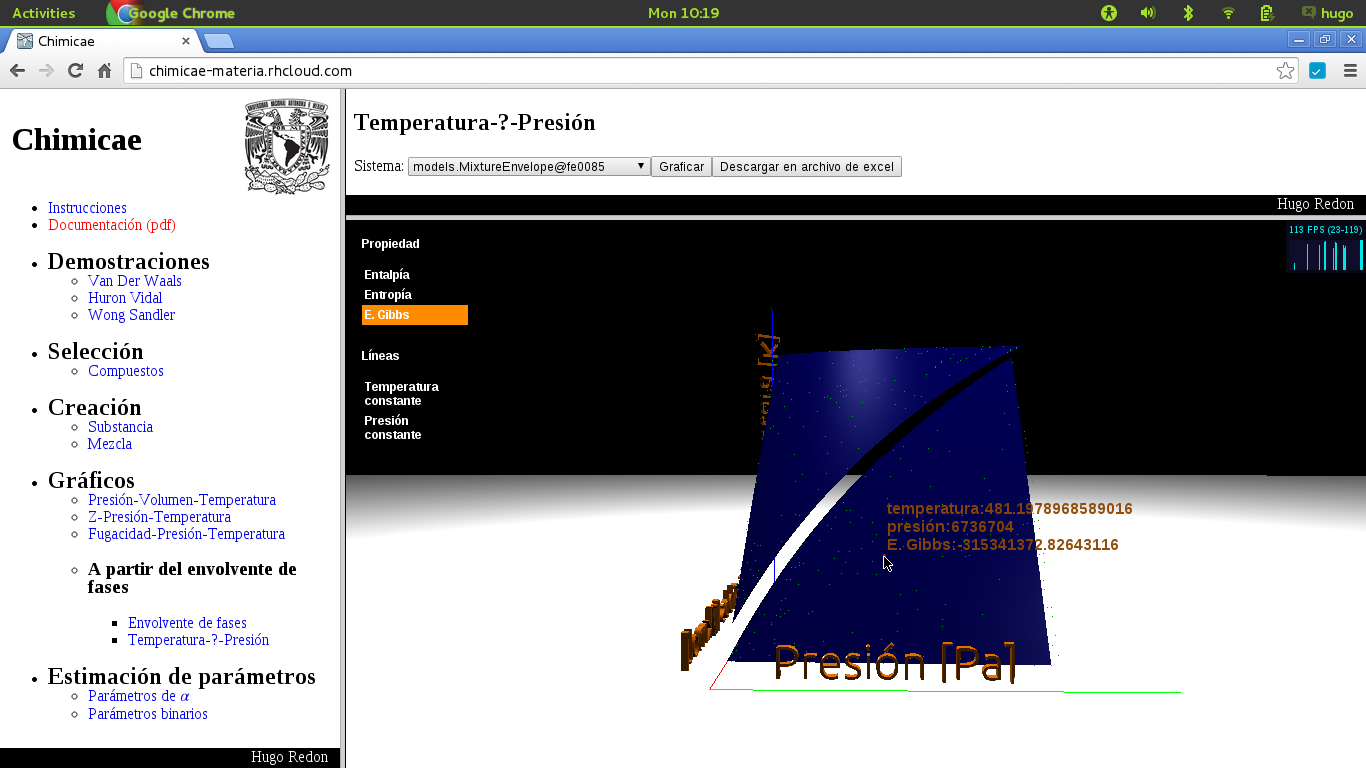
\includegraphics[scale=0.3]{waterEGPlot.png}
		\end{figure}
	\subsection{Temperatura-Presión-Volumen}\label{subsec:tpv}
		\begin{figure}[!h]
			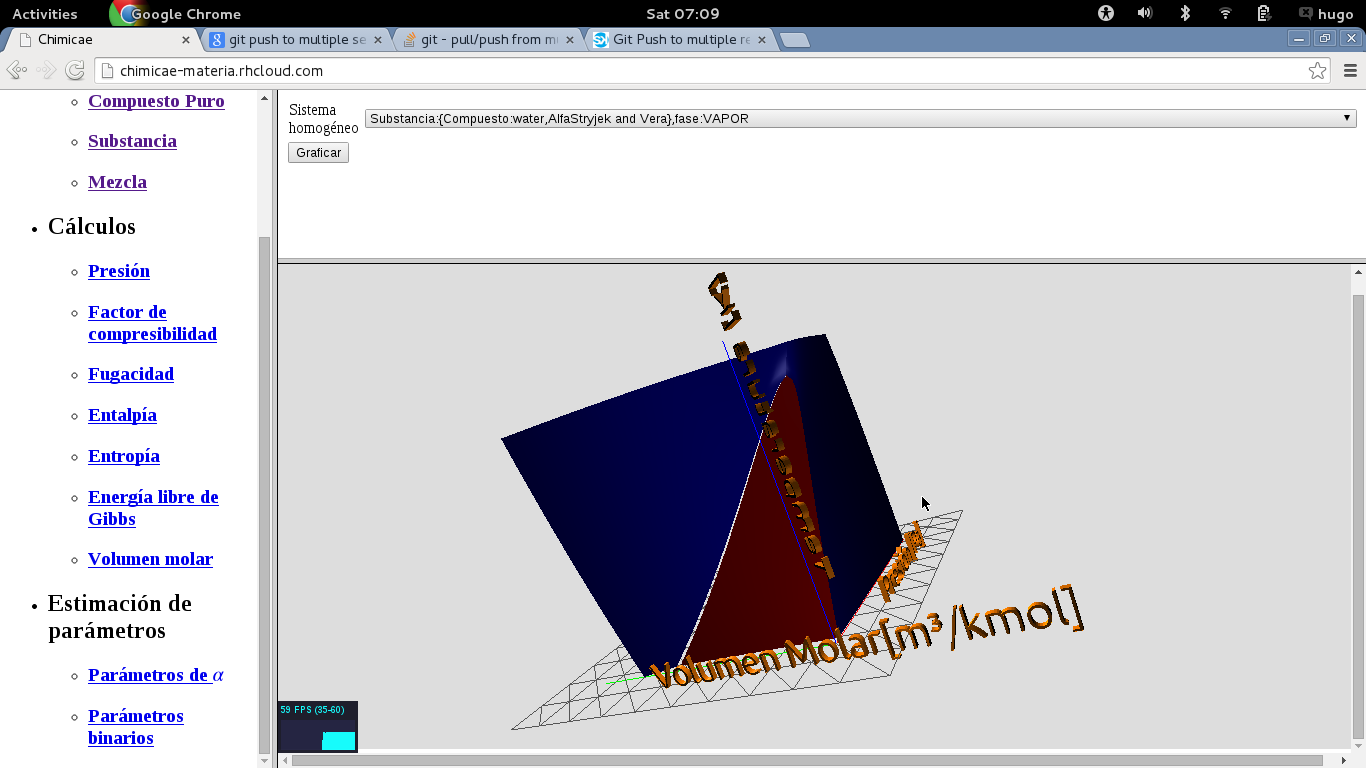
\includegraphics[scale=0.3]{waterVolumePlot.png}
		\end{figure}
	
	









\section{Estimación de parámetros de $\alpha$}\label{sec:webBinaryOptim}
\begin{figure}
	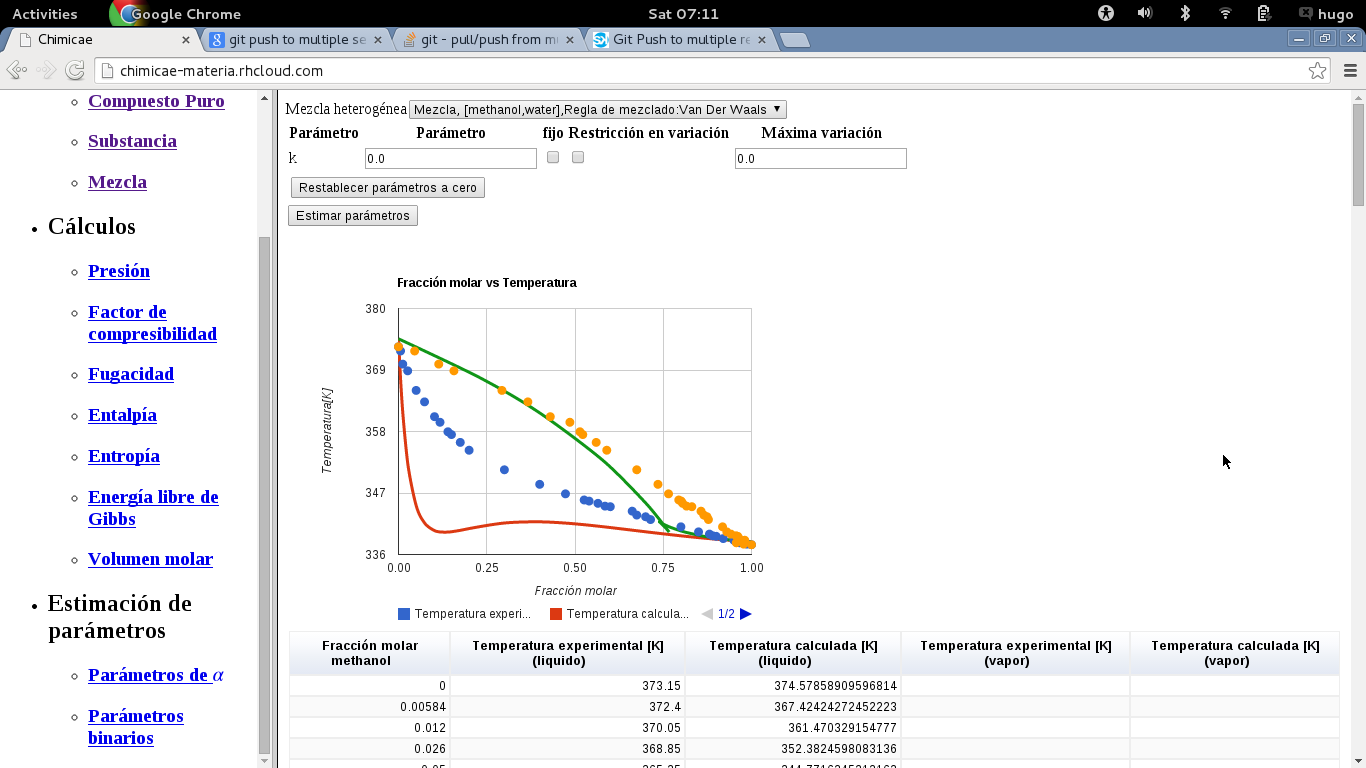
\includegraphics[scale=0.3]{waterMethanolBinaryOptPlot.png}
\end{figure}


\section{Estimación de parámetros binarios}\label{sec:webBinaryOptim}

\begin{figure}
	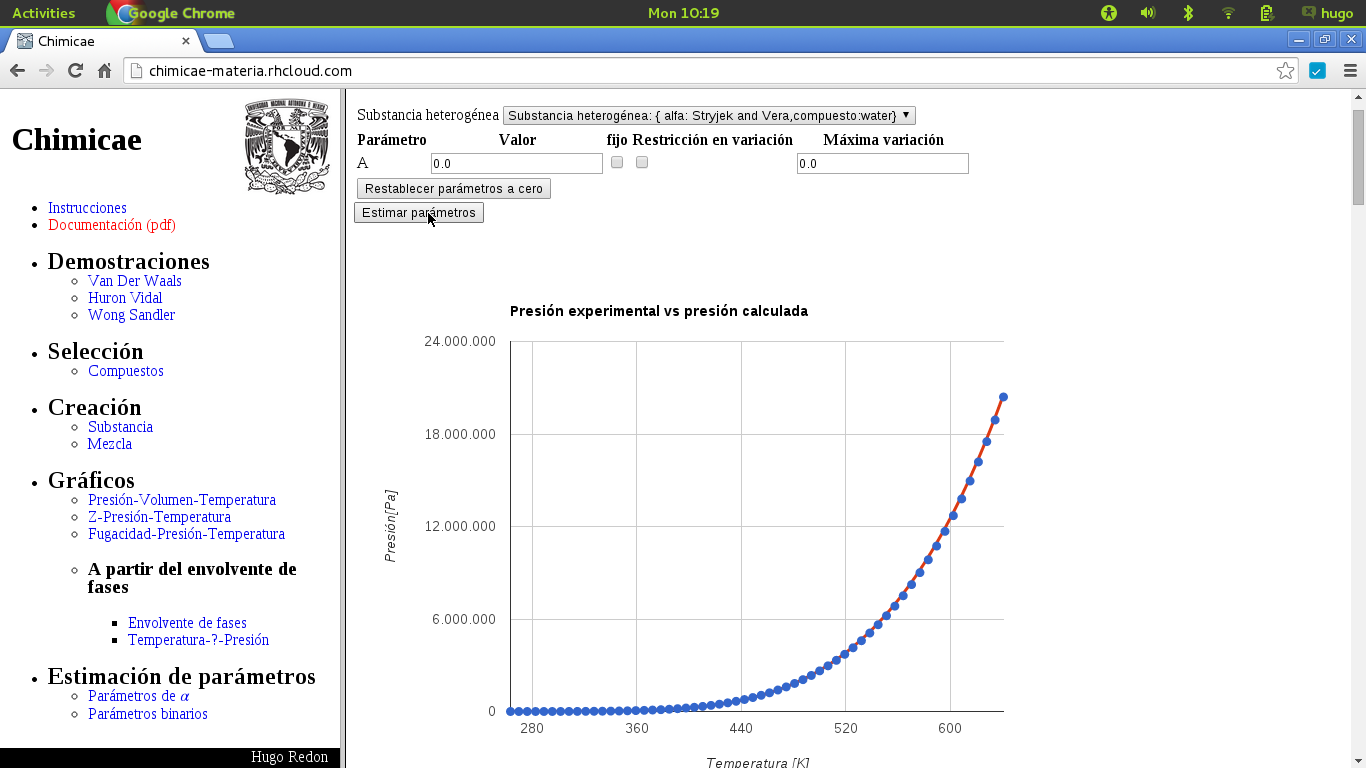
\includegraphics[scale=0.3]{waterAlphaOptPlot.png}
\end{figure}



